\documentclass[11pt,a4paper]{article}
\author{TalentSprint}
\date{}
\usepackage{fancyhdr}
\usepackage{latexsym}
\usepackage{soul}
\usepackage{verbatim}
\usepackage{graphicx}
\usepackage{array}
\usepackage{enumerate}
%\usepackage{enumitem}
\usepackage{xcolor}
\usepackage[tikz]{bclogo}
\usepackage{textcomp}
\usepackage{latexsym}
\usepackage{seqsplit} 
\usepackage{setspace}
\usepackage{listings}
\lstset{language=html,numbers=left,numberstyle=\tiny,numbersep=10pt,showstringspaces=false}
\usepackage{fancyhdr}
\headheight=14pt
\lhead{\nouppercase{}}
\rhead{\nouppercase{\leftmark}}

\graphicspath{{../Images/}}

%\pagestyle{fancy}

%========================================================================

% Lengths and widths
\addtolength{\textwidth}{2.5cm}
\addtolength{\hoffset}{0cm}
\setlength{\headsep}{-12pt} % Reduce space between header and content
\setlength{\headheight}{85pt} % If less, LaTeX automatically increases it
\renewcommand{\footrulewidth}{2pt} % Remove footer line
\renewcommand{\headrulewidth}{1pt} % Remove header line
\renewcommand{\seqinsert}{\ifmmode\allowbreak\else\-\fi} % Hyphens in seqsplit
% This two commands together give roughly
% the right line height in the tables
\renewcommand{\arraystretch}{1.3}
\onehalfspacing



% Commands
\newcommand{\SetRowColor}[1]{\noalign{\gdef\RowColorName{#1}}\rowcolor{\RowColorName}} % Shortcut for row colour
\newcommand{\mymulticolumn}[3]{\multicolumn{#1}{>{\columncolor{white}}#2}{#3}} % For coloured multi-cols
\newcolumntype{x}[1]{>{\raggedright}p{#1}} % New column types for ragged-right paragraph columns
\newcommand{\tn}{\tabularnewline} % Required as custom column type in use

% Font and Colours
\definecolor{HeadBackground}{HTML}{333333}
\definecolor{FootBackground}{HTML}{666666}
\definecolor{TextColor}{HTML}{333333}
\definecolor{DarkBackground}{HTML}{6B8E23} %{FD1AA8}
\definecolor{LightBackground}{HTML}{E8FED8} %D3FDC8
\definecolor{tit}{HTML}{FF6600}
\renewcommand{\familydefault}{\sfdefault}
\color{TextColor}
 \headsep = 25pt
% Header and Footer
\pagestyle{fancy}
\usepackage[headheight=110pt]{geometry}
\fancyhf{}% Clear header/footer

\fancyhead[r]{
\includegraphics[width = 4cm, height = 2cm]{TS-Logo.png}\hspace{0cm}}

%=================================TITLE=====================================
\fancyhead[l]{\Large{\bf{\textcolor{tit}{\textrm{Cascading Style Sheets}}}}}
%===========================================================================

\renewcommand{\headrulewidth}{0.4pt}% Default \headrulewidth is 0.4pt
\renewcommand{\footrulewidth}{0.4pt}% Default \footrulewidth is 0pt

\rfoot{Page \thepage}
\lfoot{COPYRIGHT \textcopyright TALENTSPRINT, 2015. ALL RIGHTS RESERVED.}




\begin{document}

%=================================================================================================================
\hspace{0.1cm} Cascading Style Sheets (CSS) is a fantastic tool to add layout to your websites. It saves lot of time and enables you to design websites in a different way. CSS is an important concept for people who are working on designing web pages.

Learning CSS is fun. Going further, take enough time to experiment with what you learnt in each session.
Using CSS requires basic experience with HTML. If you are not familiar with HTML, be aware of required concepts and then start using CSS.

All you need is a free and simple text editor.

For example, Microsoft Windows comes with a program called Notepad. It is usually located in Accessories in the start menu under Programs. Alternatively, you can use a similar text editor e.g., vim, scite, gedit in linux operating system.

A simple text editor is ideal for learning HTML and CSS because it doesn't affect or change the codes you type. That way, your successes and errors can only be attributed to yourself - not the software.

You can use any of the browser. We encourage you to always keep your browser updated and use the latest version.

A browser and a simple text editor is all you need.

Let's get started!

\subsection*{What is CSS?}
CSS is an acronym for Cascading Style Sheets.

CSS is a style language that defines layout of HTML documents.

For example, CSS covers fonts, colours, margins, lines, height, width, background images, advanced positions and many other things.

HTML can be (mis-)used to add layout to websites. But CSS offers more options and is more accurate and sophisticated. CSS is supported by all browsers today.

After this sessions you will be able to make your own style sheets using CSS to give your website a new great look.

\subsection*{What is the difference between CSS and HTML?}

HTML is used to \emph{structure content}. CSS is used for \emph{formatting structured content.}

As the language HTML was only used to add structure to text. An author could mark his text by stating ``this is a headline'' or ``this is a paragraph'' using HTML tags such as $<h1>$ and $<p>$.

As the Web gained popularity, designers started looking for possibilities to add layout to online documents. To meet this demand, the browser producers (at that time Netscape and Microsoft) invented new HTML tags such as for example $<font>$ which differed from the original HTML tags by defining layout - and not structure.

This also led to a situation where original structure tags such as $<table>$ were increasingly being misused to layout pages instead of adding structure to text. Many new layout tags such as $<blink>$ were only supported by one type of browser. ``You need browser X to view this page'' became a common disclaimer on web sites.

CSS was invented to remedy this situation by providing web designers with sophisticated layout opportunities supported by all browsers. At the same time, separate the presentation style of documents from the content of documents, makes site maintenance a lot easier.

\subsection*{How does CSS work?}
In this section, we will learn how to make your first style sheet. You will get to know about the basic CSS model and which codes are necessary to use CSS in an HTML document.

Many of the properties used in Cascading Style Sheets (CSS) are similar to those of HTML. Thus, if you are used to use HTML for layout, you will most likely recognize many of the codes. Let us look at a concrete example.

\underline{\textbf{Syntax:}}
\begin{center}
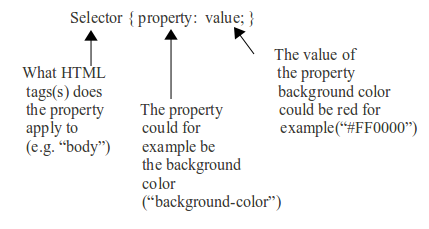
\includegraphics[height=50mm, width=110mm]{Syntax.png}
\end{center}

\begin{itemize}
\item The selector is normally the HTML element($<body>$,$<p>$,$<h>$....)you want to style.
\item It can have more than one declaration and each consists of a property and a value.
\item The property is the style attribute(color, font-size, text-align,......) you want to change. Each property has a value(yellow, 15px, center,.....).
\item  Each declarations are separated by the symbol semicolon(;)and declaration groups are surrounded by curly brackets(\{...\}).
\end{itemize}
\underline{\textbf{Example:}}\\

Applying red color as the background to a webpage:\\

\textbf{Using HTML}\\
 
\hspace{1cm} \texttt{$<$body bgcolor="\#FF0000"$>$}\\
	
\textbf{Using CSS}\\

\hspace{1cm}\texttt{body \{background-color: \#FF0000;\}}

\subsection*{Benefits of CSS}
CSS was a revolution in the world of web design. The concrete benefits of CSS include:
\begin{itemize}
\item control layout of many documents from one single style sheet.
\item more precise control of layout.
\item apply different layout to different media-types (screen, print, etc.).
\item numerous advanced and sophisticated techniques.
\end{itemize}

\subsection*{Applying CSS to an HTML Document}
When a browser reads a style sheet, it will format the document according to it. There are three ways to insert CSS to an HTML document.

There are three ways of inserting a style sheet:
\begin{itemize}
\item Inline style
\item Internal style sheet
\item External style sheet
\end{itemize}

\subsubsection*{Embedded CSS:} The $<style>$ Element

 All the CSS rules can put together in an HTML document using the $<style>$ element. This tag is placed inside $<head>...</head>$ tags. Rules defined using this syntax will be applied to all the elements available in the document.

HTML permits any number of style elements in the head section of a document.

\textbf{Syntax:}
\begin{verbatim}
     <head>
          <style type="text/css" media="...">
               Style Rules
               ............
          </style>
     </head>
\end{verbatim}
\begin{description}
\item[\emph{style}] This attribute specifies style information for the current element.
Attributes associated with $<style>$ elements are:
\item[\emph{type =} content-type]  This attribute specifies the style sheet language of the element's contents and overrides the default style sheet language. The style sheet language is specified as a content type (e.g., ``text/css''). There is no default value for this attribute; we have to assign a value for this attribute.This the required attribute.
\item[\emph{media =} media-descriptors]  This attribute specifies the intended destination medium for style information. It may be a single media descriptor or a comma-separated list. The default value for this attribute is ``screen''.
\end{description}
\underline{\textbf{Example:}}
\begin{verbatim}
     <html>
          <head>
               <style type="text/css" media="all">
                    h1{color: #DD5600;}
               </style>
          </head
          <body>
               <h1> Applying Styles to these text placed in h1 tag </h1>
               <p> These lines of text has no style.........<p>
          </body>
     </html>
\end{verbatim}
\begin{center}
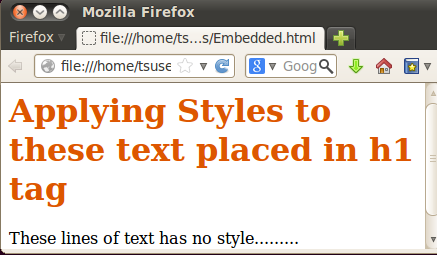
\includegraphics[scale=0.6]{Embedded}\\
\end{center}

\subsubsection*{In-line style sheet}

CSS styles can be assigned to individual HTML elements with the \emph{style} attribute,
Inline styles will have precedence over all other styles.


\subsubsection*{Syntax:}

\begin{verbatim}<tag style="property1: value; property2: value;"> </tag>\end{verbatim}
\underline{\textbf{Example:}}

\begin{verbatim}<h1 style="color: red; text-decoration: underline;">Hello</h1>\end{verbatim}

\subsubsection*{Sample Example:}

\hspace{1cm}Let's write a sample code how to use Inline style.
\begin{verbatim}
     <html>
          <head>
               <title>Inline Style Sheet</title>
          </head>
          <body style="background-color: #FF0000;">
               <p>This is a red page</p>
          </body>
     </html>
\end{verbatim}
It displays as follows:

\begin{center}
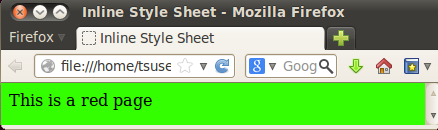
\includegraphics[scale=0.7]{InlineStyleSheet}\\
\end{center}

\begin{bclogo}[couleur=blue!5, arrondi=0.3, logo=\bctrombone]{Note}
Inline CSS should be avoided as it increases maintenance cost and blurs line between presentation and content.
\end{bclogo}


So far, we were being used CSS through the \emph{style} attribute, which is also known as inline styles, but inline styles don't separate content and style in a website. That's why internal and external style sheets are so important.

Before going further concept we have to learn about two more very important HTML tag attributes: \emph{class=``''} and \emph{id=``''}(used for identification and grouping of elements).

\subsection*{Identification and grouping of elements}
If we want to apply a special style to a particular element or a particular group of elements. In addition to setting a style for a HTML element, CSS also allows to specify your own selectors called \textbf{``id''} and \textbf{``class''}.


\subsubsection*{id Selector}
\begin{itemize}
\item The id selector is used to specify a style for a single, unique element.
\item The id selector uses the id attribute of the HTML element, and is defined with a ``\#''.
 The style rule below will be applied to the element with id=``first'':
\end{itemize}
\underline{\textbf{Example:}}
\begin{verbatim}
     <html>
          <head><title>My Webpage</title>
               <style>
                    body {background-color : #FF0000 ;}
                    #first{color : blue ; text-align : center ;}
               </style>
          </head>
          <body>
               <p id = "first">Hello World!!!</p>
               <p>This paragraph is not affected by the style.</p>
          </body>
     </html>
\end{verbatim}
\begin{center}
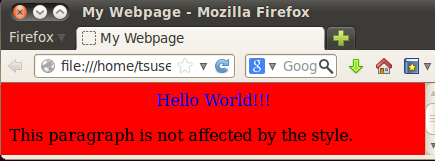
\includegraphics[scale=0.7]{IdSelector}
\end{center}

\subsubsection*{class Selector}
\begin{itemize}
\item The class selector is used to specify a style for a group of elements. Unlike the id selector, the class selector is most often used on several elements.
\item This allows you to set a particular style for many HTML elements with the same class.
\item The class selector uses the HTML class attribute, and is defined with a ``.''\\

Example below shows, all $<p>$ elements with class=``changestyle'' will be center-aligned and text color is changed to green color.\\

If we have to apply style to all the HTML elements present in the document then we have to replace \emph{``p.changestyle''} to \emph{``.changestyle''} then the style will automatically applied to all the elements in the body.
\end{itemize}
\underline{\textbf{Example:}}\\

Applying styles for the elements in the class.
\begin{verbatim}
     <html>
          <head>
               <style>
                    p.changestyle
                    {
                         text-align:center;
                         color:green;
                    }
               </style>
          </head>
          <body>
               <h1 class="changestyle">This heading will not be
                                                     affected</h1>
               <p class="changestyle">This paragraph will be 
                            center-aligned and changes its 
                                           text color to green.</p> 
          </body>
     </html>
\end{verbatim}
\begin{center}
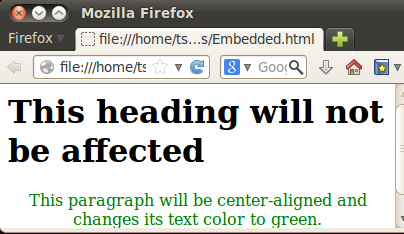
\includegraphics[scale=0.6]{ClassSelector}
\end{center}

\subsection*{Internal style sheet}

An internal style sheet should be used when a single document has a unique style. While using internal style sheet, You have to define internal styles in the head section(i.e., $<head>$) of an HTML page, by using the $<style>$ tag.


\subsubsection*{Creating an internal CSS}

CSS code is not written the same way as HTML code is. This makes sense because CSS is not HTML, but rather a way of manipulating existing HTML and finally put CSS inside style tags.The HTML code below contains an example of $<style>$'s usage.


\underline{\textbf{Example:}} Designing an internal style sheet 
\begin{verbatim}
     <html>
          <head>
               <title>Internal Style Sheet</title>
                    <style type="text/css">
                         p { color: blue; }
                         .newStyle { font-size: 20px; }
                         #change
                           {
                               font-size: 28px;
                               text-align: center;
                               color: green;
                           }
                    </style>
          </head>
          <body>
               <p>Woo hoo! I'm learning HTML!</p>
               <p class="newStyle">Woo hoo! I'm learning HTML!</p>
               <p class="newStyle" id="change">Woo hoo! I'm 
                                                learning HTML!</p>
               <p class="newStyle">Woo hoo! I'm learning HTML!</p>
          </body>
     </html>
\end{verbatim}
\begin{description}
\item[Explanation]\
\begin{verbatim}
p { color: blue; }
.newStyle { font-size: 20px; }
#change { font-size: 28px; text-align: center; color: green; }
\end{verbatim}
The first line of the internal style sheet has 3 parts.
\begin{description}
\item[selector] p\
The selector points to a certain type of HTML tag, which here are the paragraph tags or $<p>$....$</p>$.
\item[property] color
\item[value] blue
\end{description}
\end{description}
The second line of the internal style sheet also has these same three parts, but the HTML tag name out of the first part, the selector.

\begin{verbatim}.newStyle { font-size: 20px; }\end{verbatim}

Every html tag in the selector started with `` . '' to indicate that as a class name is going to be given, and rom above they given class name as \textbf{newStyle}.

So, Every HTML tag with the class name of newStyle has this style,

\texttt\{font-size: 20px;\} will be applied.

The third line of the internal style sheet again has the same three parts, but this time the selector was started with a ``\#'' to indicate that an id name is going to be given. From above they have given the id name as, \#change.

\begin{verbatim}#change{ font-size: 28px; text-align: center; color: green;}\end{verbatim}

Now, the HTML tag with the id name of change has this style,

\texttt{ font-size: 28px; text-align: center; color: green;} , will be applied to it.

As from above code we got to know that we have added three properties and values to this line of the style sheet. We can add as many properties and values into your selector as you want. That doesn't mean they will all work. CSS can be TRICKY. Some CSS properties and values will only seem to work with certain HTML tags or even in certain internet browsers.

we can also be more specific in the naming of the selectors in the internal style sheet. If we have repalced those three lines with the below lines.
\begin{verbatim}
p{ color: blue;}
p.newStyle{font-size: 20px;}
p.newStyle#Change{font-size: 28px; text-align: center; color: green;}
\end{verbatim}
Now, the second line will only apply its style to HTML paragraph tags with the class name ``newStyle'', and the third line will only apply its style to the one HTML paragraph tag with the class name ``\\newStyle'' and the id name ``change''. Above code displays as follows.

\begin{center}
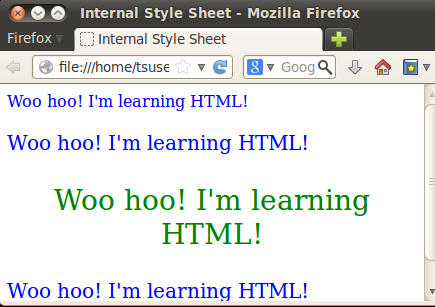
\includegraphics[scale=0.8]{InternalStyleSheet}
\end{center}
\pagebreak

\subsection*{External Style Sheet} 

When using CSS it is preferable to keep the CSS separate from your HTML. Placing CSS in a separate file allows the web designer to completely differentiate between content (HTML) and design (CSS). External CSS is a file that contains only CSS code and is saved with a ``.css'' file extension. This CSS file is then referenced in your HTML using the $<link>$ \textbf{instead} of $<style>$.

\subsubsection*{File Creation}

For example, Design an External style sheet.

Let us get started by making that external CSS file. Open up notepad.exe, or any other plain text editor and type the following CSS code.

\begin{description}
\item[CSS Code]\
\begin{verbatim}
     body { background-color: yellow; }
     p { color: white; }
     p.newStyle { font-size: 1.5px; text-align: center; }
     p.newStyle#change { font-size: 2em; text-align: right;
                                             color: blue; }
\end{verbatim}
Now save the file as a CSS (.css) file. Make sure that you are not saving it as a text (.txt) file, as notepad likes to do by default. Name the file as "test.css" (without the quotes). Now create a new HTML file and fill it with the following code.


\item[HTML Code]\
\begin{verbatim}
     <html>
          <head>
               <title>External Style Sheet</title>
                  <link rel="stylesheet" type="text/css" 
                                             href="test.css" />
          </head>
          <body>
               <p>Woo hoo! I'm learning HTML!</p>
               <p class="newStyle">Woo hoo! I'm learning HTML!</p>
               <p class="newStyle" id="change">Woo hoo! I'm
                                                learning HTML!</p>
               <p class="newStyle">Woo hoo! I'm learning HTML!</p>
          </body>
     </html>
\end{verbatim}
Then save this file as ``index.html'' (without the quotes) in the same directory as your CSS file. Now open your HTML file in your web browser and it should look something like this.
\end{description}

\subsection*{Uses:}
\begin{itemize}
\item It keeps your website design and content separate.
\item It's much easier to reuse your CSS code if you have it in a separate file. Instead of typing the same CSS code on every web page you have, simply have many pages refer to a single CSS file with the \emph{``link''} tag.
\item You can make drastic changes to your web pages with just a few changes in a single CSS file.
\end{itemize}


\subsection*{Styling Backgrounds}
\begin{center}
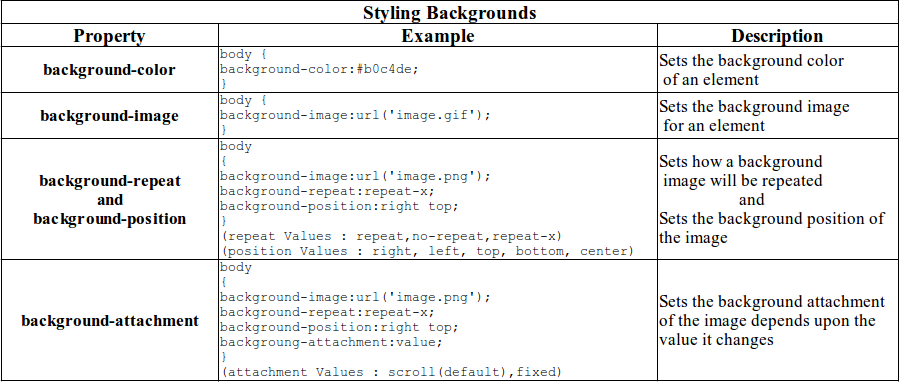
\includegraphics[width=155mm,height=85mm]{Backgrounds.png}\\
\end{center}

\subsection*{Styling Text}
\begin{center}
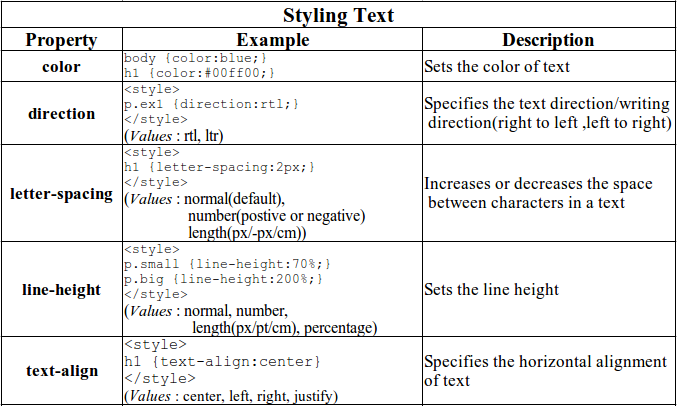
\includegraphics[scale=0.65]{first.png}
\end{center}
\begin{center}
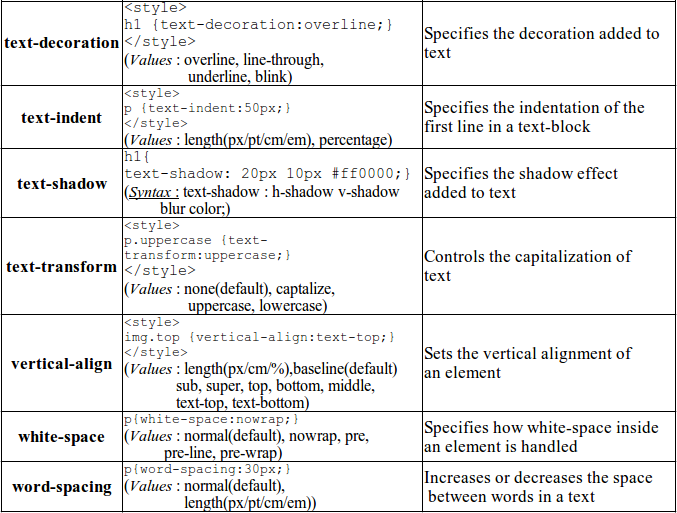
\includegraphics[width = 155mm,  height = 105mm]{Second.png}
\end{center}

\subsection*{Styling Fonts}
\begin{center}
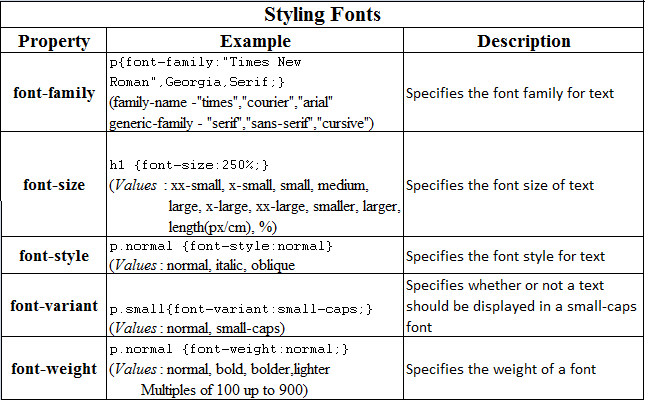
\includegraphics[width = 155mm,  height = 90mm]{Fonts.png}
\end{center}
\subsection*{Styling Links}
\begin{center}
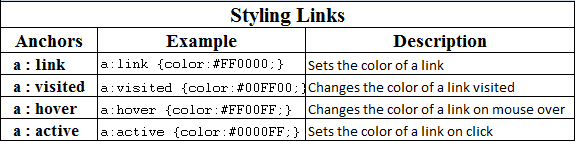
\includegraphics[width = 120mm,  height = 30mm]{Lists.png}\\
\end{center}
\subsection*{Styling Lists}
\begin{center}
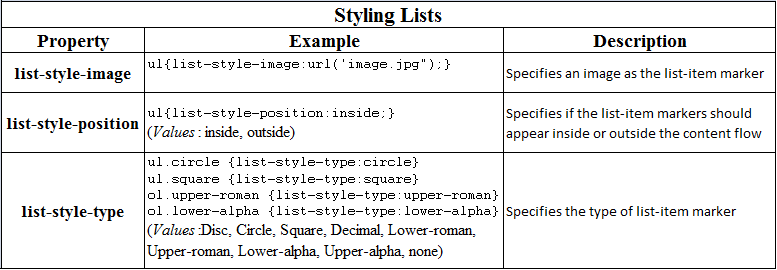
\includegraphics[width = 120mm, height = 45mm]{Links.png}\\
\end{center}
\subsection*{Styling Tables}
\begin{center}
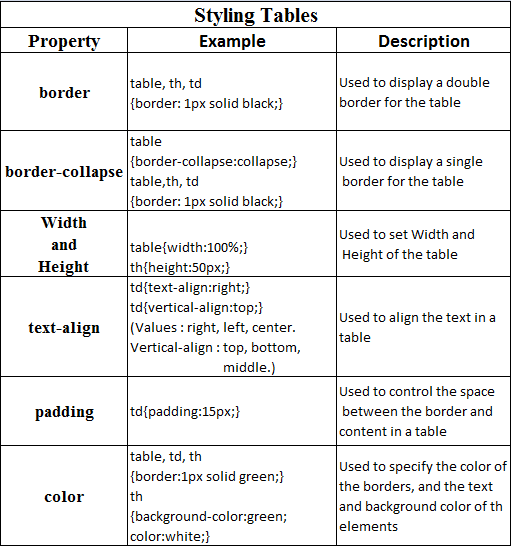
\includegraphics[width = 120mm, height = 92mm]{Tables.png}\\
\end{center}
\pagebreak
\section*{CSS Box Model}

The box model in CSS describes the boxes which are being generated for HTML-elements. The CSS box model is essentially a box that wraps around HTML elements, and it consists of: \emph{margins, borders, padding}, and the actual \emph{content}. The diagram below shows how the box model is constructed:

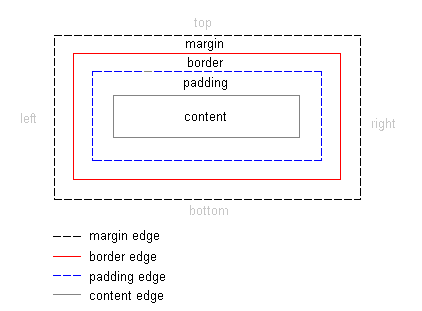
\includegraphics[scale=1.0]{Boxmodel}\\

\begin{itemize}
\item \emph{Margin} - Clears an area around the border. The margin does not have a background color, it is completely transparent
\item \emph{Border} - A border that goes around the padding and content. The border is affected by the background color of the box
\item \emph{Padding} - Clears an area around the content. The padding is affected by the background color of the box
\begin{center}
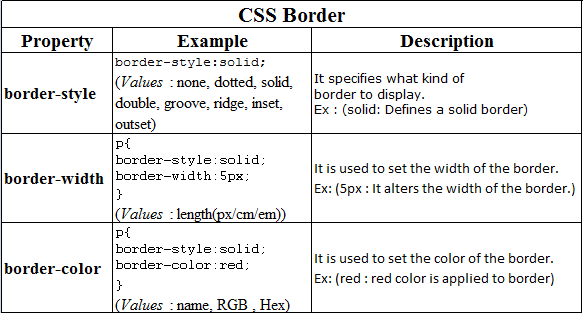
\includegraphics[width = 150mm, height = 85mm]{CSSBorder.png}\\
\end{center}
\item \emph{Content} - The content of the box, where text and images appear
\end{itemize}


\end{document}
